\documentclass[aps,pre,preprint,notitlepage,nofootinbib,superscriptaddress]{revtex4-2}

\usepackage[T1]{fontenc}
\usepackage{lmodern}
\usepackage{microtype}
\usepackage{amsmath,amssymb,mathtools,bm,mathrsfs,amsthm}
\usepackage{booktabs,array}
\usepackage{siunitx}
\usepackage{tikz}
\usetikzlibrary{arrows.meta,calc,decorations.markings,decorations.pathmorphing,decorations.pathreplacing,positioning,shapes.geometric,fit,backgrounds}
\usetikzlibrary{hobby}
\usetikzlibrary{knots,hobby,calc,arrows.meta,intersections,decorations.pathreplacing,decorations.markings,shapes.geometric,spath3}
\usepackage{hyperref}
\usepackage[nameinlink,noabbrev]{cleveref}
\usepackage{xcolor}
\usepackage{enumitem}

\hypersetup{
  colorlinks=true,
  linkcolor=blue!55!black,
  citecolor=blue!55!black,
  urlcolor=blue!55!black,
  pdftitle={Angular-Projector Normalization and Finite-Core Energetics of Tight Knotted Vortex Tubes},
  pdfauthor={Omar Iskandarani},
  pdfsubject={Normalization ambiguity, finite-core energetics, and gauge matching for tight knotted vortex tubes},
  pdfkeywords={vortex dynamics, ropelength, ideal knots, angular measure, helicity, Biot-Savart energy, naturalness, gauge coupling}
}

\sisetup{separate-uncertainty=true, per-mode=symbol}
\newcommand{\dd}{\mathrm d}
\newcommand{\RR}{\mathbb R}
\newcommand{\Rop}{\operatorname{Rop}}
\newcommand{\FP}{\operatorname{FP}}
\newcommand{\Tr}{\operatorname{Tr}}
\newcommand{\e}{\mathrm e}
\newcommand{\ii}{\mathrm i}
\newcommand{\calH}{\mathcal H}
\newcommand{\calL}{\mathcal L}
\newcommand{\calR}{\mathcal R}
\newcommand{\calI}{\mathcal I}
\newcommand{\calC}{\mathcal C}
\newcommand{\calE}{\mathcal E}
\newcommand{\calG}{\mathcal G}
\newcommand{\Rmicro}{\mathscr R_{\mathrm{micro}}}
\newcommand{\Rgeom}{\mathscr R_{0}}
\newcommand{\Reff}{\mathscr R_{\mathrm{eff}}}
\newcommand{\ZL}{Z_L}
\newcommand{\ZOmega}{Z_{\Omega}}
\newcommand{\Rnl}{\mathscr R_{\mathrm{nl}}^{\mathrm{reg}}}
\newcommand{\unitvec}[1]{\widehat{\bm #1}}

\newtheorem{proposition}{Proposition}
\newtheorem{corollary}{Corollary}
\newtheorem{hypothesis}{Matching hypothesis}
\newtheorem{remark}{Remark}




\begin{document}

\title{\texorpdfstring{Angular-Projector Normalization and Finite-Core Energetics of Tight Knotted Vortex Tubes\\\large Why a trefoil-length coincidence does not yet determine a gauge coupling}{Angular-Projector Normalization and Finite-Core Energetics of Tight Knotted Vortex Tubes: Why a trefoil-length coincidence does not yet determine a gauge coupling}}

\author{Omar Iskandarani}
\email{info@omariskandarani.com}
\thanks{ORCID: 0009-0006-1686-3961  DOI: 10.5281/zenodo.21792160}
\affiliation{Independent Researcher, Groningen, The Netherlands}
\date{2 August 2026; manuscript version 0.2.1}

\begin{abstract}
For a unit tangent $\bm t$ and the incompressible transverse projector $P_{ij}=\delta_{ij}-\widehat{k}_i\widehat{k}_j$, rotational invariance gives the exact normalized identity
\[
\frac{1}{4\pi}\int_{S^2}t_iP_{ij}t_j\,\dd\Omega=\frac23.
\]
The corresponding unnormalized integral is $8\pi/3$.  This paper distinguishes that exact geometric statement from the additional convention needed to use $8\pi/3$ as a physical coefficient multiplying a diameter-normalized tube length.  In a Fourier-space field calculation the angular integral is accompanied by a radial spectral measure, powers of $2\pi$, field normalization, and source normalization.  Transversality alone fixes the fraction $2/3$, not the total measure carried by a response functional.

Two local no-go results remain exact.  The bare isotropic projector contains no curvature, torsion, or contact information, and the term linear in curvature in the Jacobian of a constant-radius tube vanishes after integration around the cross-section.  Neither construction generates a finite-core correction.  Starting from the Euler kinetic energy, the vorticity and Biot--Savart representations are derived.  The finite-core energy is then shown to contain a nonanalytic logarithmic self-energy and genuinely nonlocal terms.  A purely polynomial expansion in $D\kappa$ is not controlled for a tight trefoil because $D\kappa$ reaches $2$ on finite curvature-limited intervals.

Helicity constrains a framed tube through $\mathcal H/\Gamma^2=SL=Wr+Tw$, while the standard quadratic variational bound gives
\[
\mathcal I_{\Omega^2}\geq \frac{4\pi^2}{\mathcal L_D}(SL-Wr)^2.
\]
The bound is parity even, but its numerical value depends strongly on the independently chosen self-linking sector.  A naturalness audit shows that, in a commonly used dimensionless curvature basis, closing the trefoil residual requires coefficients of order $10^{-2}$--$10^{-3}$ rather than order unity; this is a diagnostic of suppression in that basis, not a universal theorem.

The numerical provenance is also corrected.  The high-resolution study reports a polygonal length $L_p$, an inscribed-curve upper bound $L_c$, and a weighted estimate $L_a$; these quantities have different epistemic status.  Their internal spread is far smaller than the separation between the high-resolution and rounded Fourier branches, which is itself about eighty times smaller than the external residual.  Finally, a gauge interpretation is retained only as an open matching hypothesis requiring independent source normalization, a protected $U(1)$ constraint, two physical transverse modes, static--radiative universality, and one Lorentz-invariant infrared causal cone shared with matter.  The trefoil number is therefore a normalization-dependent geometric coincidence and a falsification target, not a derived fine-structure constant.
\end{abstract}

\keywords{vortex dynamics, ropelength, ideal knots, transverse projector, angular measure, helicity, writhe, twist, Biot--Savart energy, logarithmic self-energy, naturalness, gauge coupling}

\maketitle

\section{Introduction}

Knotted tubes appear in fluid dynamics, magnetohydrodynamics, elasticity, polymer physics, and flux-tube models.  Across these subjects one repeatedly encounters a leading contribution proportional to tube length, supplemented by framing, curvature, contact, or nonlocal terms.  Such structures are established in the magnetic-knot literature and in models of tightly knotted flux tubes \cite{ChuiMoffatt1995,MaggioniRicca2009,BuniyKephart2005,BuniyEtAl2014}.  Hydrodynamic vortex knots likewise possess nontrivial velocity, energy, and helicity that depend on winding and nonlocal induction \cite{MaggioniEtAl2009,MaggioniEtAl2010}.

The present paper addresses a narrower question.  For the incompressible transverse projector, the unnormalized angular integral of the transverse tangent fraction is $8\pi/3$.  When multiplied by the diameter-normalized ropelength of a high-resolution trefoil, this produces a number near the inverse low-energy electromagnetic coupling.  The arithmetic is correct.  The physical interpretation is not automatic, because an angular integral is not yet a normalized response coefficient.  The full spectral measure, radial weight, subtraction prescription, field normalization, and source normalization must be derived from one microscopic calculation.

The purpose of this revision is therefore diagnostic rather than confirmatory.  It separates:
\begin{enumerate}[label=(\roman*)]
  \item the exact normalized angular mean $2/3$;
  \item the convention-dependent unnormalized value $8\pi/3$;
  \item local geometric identities that cannot generate a correction;
  \item the logarithmic and nonlocal structure of finite-core vortex energy;
  \item the absence of a small-curvature parameter for a tight trefoil;
  \item helicity and framing constraints;
  \item the extra requirements for an electromagnetic gauge interpretation.
\end{enumerate}

No direct calculation of the fine-structure constant is claimed.  The external value is consulted only after all geometric, normalization, core, and framing choices have been fixed.  In particular, a chosen angular normalization or subtraction convention is not promoted to a physical theorem merely because it produces a nearby number.

Ropelength minimizers exist in every tame knot type and are generally $C^{1,1}$ rather than necessarily $C^2$ \cite{CantarellaKusnerSullivan2002}.  Constrained-gradient calculations expose active struts and kinks \cite{AshtonCantarellaPiatekRawdon2011}.  The high-resolution trefoil exhibits six finite curvature-limited intervals, discontinuous-curvature conjectures, singular torsional structure, and a nontrivial contact map \cite{PrzybylPieranski2014}.  Those features make it an unusually severe test of any local derivative expansion.

\section{Geometric preliminaries and conventions}
\label{sec:geometry}

Let $\gamma:S^1\to\RR^3$ be a closed embedded curve parameterized by arclength $s$, with unit tangent
\begin{equation}
  \bm t(s)=\frac{\dd\bm\gamma}{\dd s},\qquad |\bm t|=1.
\end{equation}
Let $a$ denote the radius of an embedded normal tube and let $D=2a$.  The standard radius-normalized ropelength and the diameter-normalized length are
\begin{equation}
  \Rop_a[\gamma]=\frac{L}{a},\qquad
  \calL_D[\gamma]=\frac{L}{D}=\frac12\Rop_a[\gamma].
  \label{eq:diameter-normalized-v020}
\end{equation}
The factor-of-two conversion is essential: the high-resolution trefoil value near $32.743$ is radius normalized, while the value near $16.3715$ is diameter normalized.


        \begin{table}[h!]
            \centering
            \label{tab:trefoil-variants}
            \begin{tabular}{c c}
                \textbf{$T_{(3,2)}$ Left handed}  & \textbf{Right handed $T_{(2,3)}$} \\
                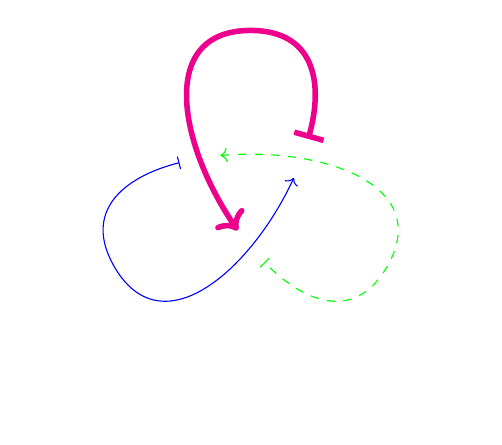
\begin{tikzpicture}
                    \path[spath/save=trefoil]
                    (0,2) .. controls +(2.2,0) and +(120:-2.2) ..
                    (210:2) .. controls +(120:2.2) and +(60:2.2) ..
                    (-30:2) .. controls +(60:-2.2) and +(-2.2,0) .. (0,2);
                    \tikzset{
                        every trefoil component/.style={draw},
                        trefoil component 1/.style={blue, <-|},
                        trefoil component 2/.style={green, dashed, <-|},
                        trefoil component 3/.style={magenta, line width=2pt,  <-|},
                        spath/knot={trefoil}{15pt}{1,3,5},
                    }
                \end{tikzpicture}
                &
                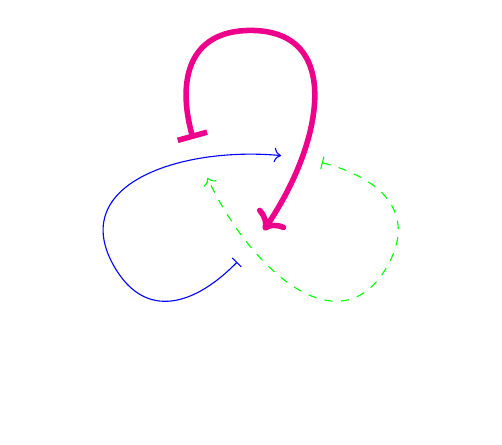
\begin{tikzpicture}
                    \path[spath/save=trefoil]
                    (0,2) .. controls +(2.2,0) and +(120:-2.2) ..
                    (210:2) .. controls +(120:2.2) and +(60:2.2) ..
                    (-30:2) .. controls +(60:-2.2) and +(-2.2,0) .. (0,2);
                    \tikzset{
                        every trefoil component/.style={draw},
                        trefoil component 1/.style={blue, |->},
                        trefoil component 2/.style={green, dashed, |->},
                        trefoil component 3/.style={magenta, line width=2pt, |->},
                        spath/knot={trefoil}{15pt}{2,4,6},
                    }
                \end{tikzpicture}
            \end{tabular}
        \end{table}



    \begin{figure}[t]
\centering
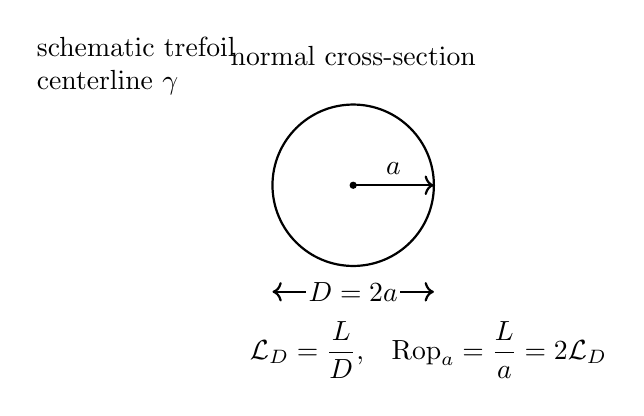
\begin{tikzpicture}[scale=0.82]

  \node[align=left,anchor=west] at (3.15,2.0)
    {schematic trefoil\\centerline $\gamma$};
  \begin{scope}[shift={(8.2,0.15)}]
    \draw[thick] (0,0) circle (1.25);
    \draw[<->,thick] (-1.25,-1.65)--(1.25,-1.65)
      node[midway,fill=white,inner sep=1pt] {$D=2a$};
    \draw[->,thick] (0,0)--(1.25,0)
      node[midway,above] {$a$};
    \fill (0,0) circle (1.6pt);
    \node[align=center] at (0,2.0) {normal cross-section};
    \node[align=left,anchor=west] at (-1.75,-2.55)
      {$\displaystyle \calL_D=\frac{L}{D}$,\quad
       $\displaystyle \Rop_a=\frac{L}{a}=2\calL_D$};
  \end{scope}
\end{tikzpicture}
\caption{A schematic trefoil centerline and the radius--diameter convention.  The plotted trefoil is not a numerical ropelength minimizer; it only illustrates the topology and normalization.}
\label{fig:trefoil-convention}
\end{figure}

For a $C^{1,1}$ minimizer, curvature exists almost everywhere and is essentially bounded.  A physical twist variable should be attached to a material or core director; unregularized Frenet torsion is not sufficient at inflection points, curvature discontinuities, or frame jumps.

\section{Normalized and unnormalized transverse-projector identities}
\label{sec:projector}

In Fourier space, incompressibility requires $k_i\widetilde u_i(\bm k)=0$.  The orthogonal projector onto the plane transverse to $\bm k$ is
\begin{equation}
  P_{ij}(\unitvec{k})=\delta_{ij}-\widehat k_i\widehat k_j.
  \label{eq:projector-v020}
\end{equation}
For a fixed unit tangent,
\begin{equation}
  t_iP_{ij}t_j=1-(\bm t\cdot\unitvec{k})^2.
\end{equation}
Rotational invariance gives
\begin{equation}
  \int_{S^2}\widehat k_i\widehat k_j\,\dd\Omega
  =\frac{4\pi}{3}\delta_{ij}.
\end{equation}

\begin{proposition}[Normalized transverse fraction]
For every unit vector $\bm t\in\RR^3$,
\begin{equation}
  \boxed{
  \left\langle t_iP_{ij}t_j\right\rangle_{S^2}
  :=\frac{1}{4\pi}\int_{S^2}t_iP_{ij}t_j\,\dd\Omega
  =\frac23.}
  \label{eq:normalized-23}
\end{equation}
Equivalently,
\begin{equation}
  \boxed{\int_{S^2}t_iP_{ij}t_j\,\dd\Omega=\frac{8\pi}{3}.}
  \label{eq:unnormalized-8pi3}
\end{equation}
\end{proposition}

\begin{proof}
Using isotropy,
\begin{align}
  \int_{S^2}t_iP_{ij}t_j\,\dd\Omega
  &=4\pi-t_it_j\frac{4\pi}{3}\delta_{ij}
  =4\pi-\frac{4\pi}{3}|\bm t|^2
  =\frac{8\pi}{3}.
\end{align}
Division by $4\pi$ gives $2/3$.
\end{proof}

The factor $3$ is the denominator of the isotropic second moment in three spatial dimensions.  It has no relation to the trefoil crossing number or threefold symmetry.





    \paragraph{The transverse projector removes the component of $\bm t$ parallel to $\unitvec{k}$.  The normalized isotropic mean is $2/3$.  Multiplication by the total solid angle $4\pi$ gives the unnormalized integral $8\pi/3$; retaining that factor in a physical response requires an independently derived measure normalization.}







\subsection{Measure normalization is additional physics}

Let $\mu$ be the angular part of a physical spectral measure.  Define
\begin{equation}
  \calG_\mu[\gamma]
  :=\int_\gamma\frac{\dd s}{D}
  \int_{S^2}t_iP_{ij}t_j\,\dd\mu(\unitvec{k}).
\end{equation}
For an isotropic measure $\dd\mu=C_\Omega\,\dd\Omega/(4\pi)$,
\begin{equation}
  \calG_\mu[\gamma]=\frac23 C_\Omega\calL_D.
  \label{eq:general-measure}
\end{equation}
The unnormalized choice $\dd\mu=\dd\Omega$ corresponds to $C_\Omega=4\pi$ and reproduces $(8\pi/3)\calL_D$.  A normalized angular probability measure corresponds to $C_\Omega=1$ and gives $(2/3)\calL_D$.

Steradians are dimensionless in SI, so this is not a dimensional inconsistency.  It is a normalization ambiguity.  In a field calculation, the angular integral normally appears inside a full momentum measure such as $\dd^3k/(2\pi)^3$, together with radial weights, dispersion, eigenmode normalization, and subtraction terms.  None of those factors is supplied by the projector identity.  We therefore write the physical leading line contribution as
\begin{equation}
  \boxed{\mathscr R_{\rm line}=\ZL(\mu)\calL_D,}
  \label{eq:open-line-coefficient}
\end{equation}
where $\ZL(\mu)$ must be independently matched.  The numerical choice $\ZL=8\pi/3$ is a candidate convention, not a consequence of incompressibility alone.

\subsection{Local projector no-go}

The normalized and unnormalized angular results are constant for every unit tangent.  Therefore neither contains local curvature, torsion, writhe, contact, or profile information:
\begin{equation}
  \boxed{\Delta_{\rm bare\ projector}=0.}
\end{equation}
A geometry-sensitive correction requires a modified kernel, a core-resolved field, a material frame, or nonlocal interaction.

\section{Constant-radius tube volume: identity and limitation}
\label{sec:tube-volume}

For a smooth portion of a centerline, Frenet tube coordinates give
\begin{equation}
  \bm x(s,r,\phi)=\bm\gamma(s)
  +r\cos\phi\,\bm n(s)+r\sin\phi\,\bm b(s),
\end{equation}
with Jacobian
\begin{equation}
  \dd V=r\left(1-\kappa r\cos\phi\right)
  \dd r\,\dd\phi\,\dd s.
\end{equation}
For the open tube $0\le r<a$ before loss of normal injectivity,
\begin{equation}
  V_{\rm tube}=\pi a^2L,
\end{equation}
because the term linear in curvature integrates to zero around the cross-section.

One may then write
\begin{equation}
  \frac{4}{3}\frac{V_{\rm tube}}{a^3}
  =\frac{8\pi}{3}\frac{L}{D}.
  \label{eq:tube-restatement}
\end{equation}
This is not a second derivation of $8\pi/3$: the prefactor $4/3$ has been selected so that the right-hand side reproduces the same coefficient.  Equation~\eqref{eq:tube-restatement} is an algebraic restatement of the chosen normalization.

\begin{remark}[Boundary of validity]
The coordinate map is regular only for $1-\kappa r\cos\phi>0$ in the open tube.  A tight tube reaches $a\kappa_{\max}=1$ at curvature-limited points, and its boundary also touches itself on the contact set.  The volume formula is therefore understood as the volume of the embedded open tube or as a limiting statement.  It cannot by itself describe boundary contact stress or core deformation.
\end{remark}

The curvature cancellation nevertheless supplies a robust no-go result:
\begin{equation}
  \boxed{\Delta_{\rm constant\ circular\ volume}=0.}
\end{equation}
A nonzero tube-based correction requires profile variation, cross-sectional deformation, contact stress, overlap regularization, or additional dynamics.

\section{Euler energy, Biot--Savart form, and finite-core logarithms}
\label{sec:euler-energy}

For an incompressible fluid of constant density $\rho$,
\begin{equation}
  E=\frac{\rho}{2}\int |\bm u(\bm x)|^2\,\dd^3x,
  \qquad \nabla\cdot\bm u=0.
\end{equation}
With vorticity $\bm\omega=\nabla\times\bm u$ and suitable decay or boundary conditions,
\begin{equation}
  \boxed{
  E=\frac{\rho}{8\pi}
  \int\!\dd^3x\int\!\dd^3x'\,
  \frac{\bm\omega(\bm x)\cdot\bm\omega(\bm x')}
       {|\bm x-\bm x'|}.}
  \label{eq:vorticity-energy-v020}
\end{equation}
For a formal zero-radius filament,
\begin{equation}
  \bm\omega(\bm x)=\Gamma\oint_\gamma
  \bm t(s)\delta^{(3)}(\bm x-\bm\gamma(s))\,\dd s,
\end{equation}
which gives
\begin{equation}
  E_{\rm BS}[\gamma]
  =\frac{\rho\Gamma^2}{8\pi}
  \oint\!\oint
  \frac{\bm t(s)\cdot\bm t(s')}
       {|\bm\gamma(s)-\bm\gamma(s')|}\,\dd s\,\dd s'.
  \label{eq:filament-energy-v020}
\end{equation}
The diagonal diverges.  A physical result requires a resolved vorticity distribution or an explicit regularization.

For a slender vortex ring of major radius $R$ and core radius $a$, the standard finite-core asymptotics has the structure \cite{Saffman1992}
\begin{equation}
  E_{\rm ring}
  =\frac12\rho\Gamma^2R
   \left[\ln\!\left(\frac{8R}{a}\right)-C_f+o(1)\right],
  \qquad a/R\to0,
  \label{eq:ring-log}
\end{equation}
where $C_f$ depends on the core profile.  In terms of $\widehat\kappa=D\kappa=2a/R$, the logarithm is $\ln(16/\widehat\kappa)$.  Thus the leading finite-core structure contains a contribution schematically proportional to
\begin{equation}
  \calL_D\ln\!\left(\frac{C}{\widehat\kappa}\right),
  \label{eq:log-line-term}
\end{equation}
not merely a polynomial in $\widehat\kappa^2$.

For a general knot there is no unique local outer cutoff $R$.  The regularized energy depends on global geometry and contact.  A safe decomposition is
\begin{equation}
  \boxed{
  \calE_f[\gamma]
  =\ZL(\mu)\calL_D
  +\Rnl[\gamma,f;\mu]
  +\Delta_{\rm local}[\gamma,f,\Omega_3;\mu],}
  \label{eq:safe-decomposition}
\end{equation}
where $\Rnl$ retains the logarithmic self-energy, long-range induction, and contact-sensitive terms rather than forcing them into a low-order polynomial.

\section{Relation to established energy--ropelength models}
\label{sec:prior-art}

Energy functionals for knotted tubes predate the present numerical coincidence.  Chui and Moffatt calculated energy and helicity for knotted magnetic flux tubes under circular and axially uniform assumptions \cite{ChuiMoffatt1995}.  Maggioni and Ricca derived a constrained minimum magnetic energy depending explicitly on ropelength and framing \cite{MaggioniRicca2009}.  Hydrodynamic calculations have compared kinetic energy and helicity across vortex knots and unknots under Biot--Savart evolution \cite{MaggioniEtAl2009,MaggioniEtAl2010}.

Length-proportional mass or energy spectra have also been proposed for tightly knotted flux tubes in high-energy models \cite{BuniyKephart2005,BuniyEtAl2014}.  Those works establish relevant precedent for the structural idea ``length plus corrections'', but they do not provide an electromagnetic derivation of the coefficient in Eq.~\eqref{eq:open-line-coefficient}.  The specific observation examined here is the numerical proximity of one unnormalized angular convention times the tight-trefoil length to an inverse electromagnetic coupling.  Its novelty, if any, lies in that numerical comparison and in the obstruction analysis, not in the general idea that knotted-tube energy may depend on ropelength and framing.

\section{Effective response and the absence of a controlled tight-knot expansion}
\label{sec:effective-expansion}

Let
\begin{equation}
  \widehat\kappa=D\kappa,
  \qquad \widehat\Omega=D\Omega_3,
\end{equation}
and define
\begin{equation}
  \calI_{\kappa^2}=\int\widehat\kappa^2\frac{\dd s}{D},
  \qquad
  \calI_{\Omega^2}=\int\widehat\Omega^2\frac{\dd s}{D}.
\end{equation}
If $\widehat\kappa\ll1$ and derivatives are small, a local expansion may supplement Eq.~\eqref{eq:safe-decomposition}:
\begin{equation}
  \Delta_{\rm local}
  =c_\kappa\calI_{\kappa^2}
  +c_\Omega\calI_{\Omega^2}
  +c_{\kappa4}\calI_{\kappa^4}
  +c_{\partial\kappa}\calI_{(\partial\kappa)^2}
  +\cdots.
  \label{eq:local-expansion-v020}
\end{equation}
This expansion is not controlled for a tight trefoil.  In the radius-one convention used by the high-resolution study, $\kappa=1$ on six finite intervals \cite{PrzybylPieranski2014}.  Since $D=2$, those intervals have
\begin{equation}
  \boxed{\widehat\kappa=D\kappa=2.}
  \label{eq:kappa-two}
\end{equation}
Consequently $\widehat\kappa^2=4$, $\widehat\kappa^4=16$, and higher local powers are not parametrically ordered.  Contact and logarithmic nonlocality are simultaneously active.  A three-operator truncation may still be tested as a phenomenological regression model, but not described as a systematic leading-order effective expansion over the complete tight knot.

\subsection{Status of the length subtraction}

Writing
\begin{equation}
  \Reff=\frac{8\pi}{3}\calL_D+c_L\calL_D+\cdots
\end{equation}
contains an exact degeneracy.  The convention
\begin{equation}
  \boxed{c_L=0}
  \label{eq:cL-convention-v020}
\end{equation}
is useful only as a preregistered subtraction rule after choosing $\ZL(\mu_0)=8\pi/3$ at a reference scheme $\mu_0$.  It prevents post hoc refitting of the length coefficient, but it does not derive the physical value of $\ZL$.  A different independently derived spectral measure could produce a different $\ZL$ while leaving the normalized projector identity unchanged.


\begin{figure}[t]
\centering
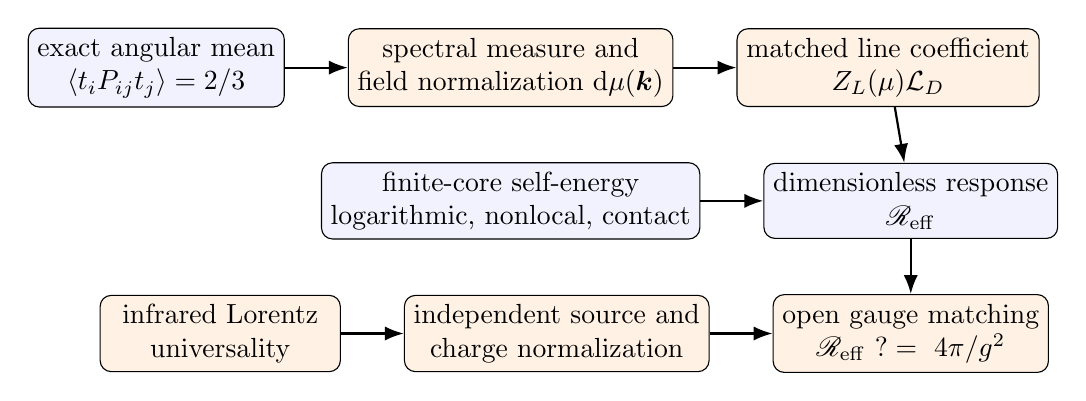
\begin{tikzpicture}[
  node distance=7mm and 8mm,
  box/.style={draw,rounded corners,align=center,minimum width=3.05cm,minimum height=0.95cm,fill=blue!5},
  open/.style={draw,rounded corners,align=center,minimum width=3.05cm,minimum height=0.95cm,fill=orange!10},
  arrow/.style={-{Latex[length=2.4mm]},thick}
]
  \node[box] (mean) {exact angular mean\\$\langle t_iP_{ij}t_j\rangle=2/3$};
  \node[open,right=of mean] (measure) {spectral measure and\\field normalization $\dd\mu(\bm k)$};
  \node[open,right=of measure] (line) {matched line coefficient\\$\ZL(\mu)\calL_D$};
  \node[box,below=of measure] (core) {finite-core self-energy\\logarithmic, nonlocal, contact};
  \node[box,right=of core] (resp) {dimensionless response\\$\Reff$};
  \node[open,below=of resp] (gauge) {open gauge matching\\$\Reff\ ?=\ 4\pi/g^2$};
  \node[open,left=of gauge] (source) {independent source and\\charge normalization};
  \node[open,left=of source] (lorentz) {infrared Lorentz\\universality};
  \draw[arrow] (mean)--(measure);
  \draw[arrow] (measure)--(line);
  \draw[arrow] (line)--(resp);
  \draw[arrow] (core)--(resp);
  \draw[arrow] (resp)--(gauge);
  \draw[arrow] (source)--(gauge);
  \draw[arrow] (lorentz)--(source);
\end{tikzpicture}
\caption{Logical separation of the exact normalized angular identity, the open spectral-measure normalization, finite-core energy, source normalization, Lorentz universality, and the optional gauge-stiffness interpretation.  The value $8\pi/3$ corresponds to one unnormalized angular convention; it is not fixed by transversality alone.}
\label{fig:logic-v020}
\end{figure}


\section{Helicity, writhe, twist, and framing sectors}
\label{sec:helicity}

The helicity of an incompressible flow is
\begin{equation}
  \calH=\int \bm u\cdot\bm\omega\,\dd^3x.
\end{equation}
For one isolated framed thin tube with circulation $\Gamma$ and no reconnection,
\begin{equation}
  \frac{\calH}{\Gamma^2}=SL=Wr+Tw
  \label{eq:calugareanu-v020}
\end{equation}
under the standard slender-tube hypotheses
\cite{Moffatt1969,MoffattRicca1992,Calugareanu1961,White1969}.  The writhe of the centerline is the Gauss integral
\begin{equation}
  Wr[\gamma]=\frac{1}{4\pi}
  \oint\!\oint
  \frac{(\bm\gamma(s)-\bm\gamma(s'))\cdot
        [\bm t(s)\times\bm t(s')]}
       {|\bm\gamma(s)-\bm\gamma(s')|^3}
  \dd s\,\dd s'.
  \label{eq:writhe-v020}
\end{equation}
Writhe is a nonlocal property of the centerline.  Twist requires a physical material director $\bm d_1\perp\bm t$:
\begin{equation}
  \Omega_3=(\bm t\times\bm d_1)\cdot\frac{\dd\bm d_1}{\dd s},
  \qquad
  Tw=\frac{1}{2\pi}\oint\Omega_3\,\dd s.
  \label{eq:material-twist-v020}
\end{equation}
This definition remains meaningful where a Frenet frame is singular or discontinuous, provided the physical material framing is specified.

\begin{figure}[t]
\centering
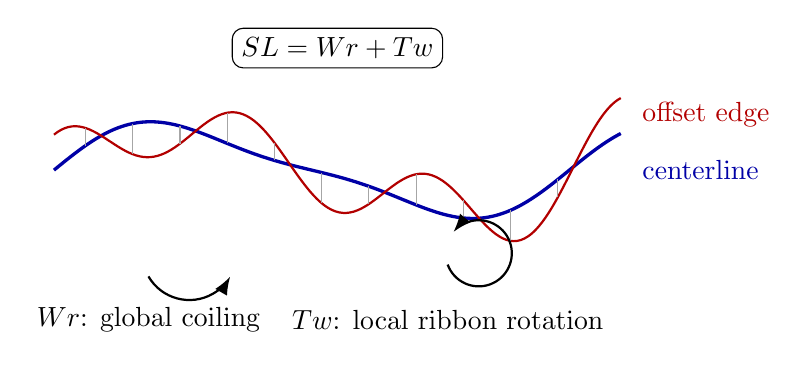
\begin{tikzpicture}[scale=1.0,>=Latex]
  \draw[very thick,blue!65!black,domain=0:7.2,samples=160,smooth,variable=\x]
    plot ({\x},{0.55*sin(55*\x)+0.15*sin(110*\x)});
  \draw[thick,red!70!black,domain=0:7.2,samples=160,smooth,variable=\x]
    plot ({\x},{0.55*sin(55*\x)+0.15*sin(110*\x)+0.45*cos(150*\x)});
  \foreach \x in {0.4,1.0,...,7.0}{
    \pgfmathsetmacro{\yc}{0.55*sin(55*\x)+0.15*sin(110*\x)}
    \pgfmathsetmacro{\yo}{0.45*cos(150*\x)}
    \draw[gray!70] (\x,\yc)--(\x,\yc+\yo);
  }
  \node[blue!65!black,anchor=west] at (7.35,0.0) {centerline};
  \node[red!70!black,anchor=west] at (7.35,0.7) {offset edge};
  \draw[->,thick] (1.2,-1.35) arc[start angle=210,end angle=330,radius=0.6];
  \node at (1.2,-1.9) {$Wr$: global coiling};
  \draw[->,thick] (5.0,-1.2) arc[start angle=200,end angle=500,radius=0.42];
  \node at (5.0,-1.9) {$Tw$: local ribbon rotation};
  \node[draw,rounded corners,fill=white] at (3.6,1.55) {$SL=Wr+Tw$};
\end{tikzpicture}
\caption{Schematic ribbon representation of self-linking.  Writhe is a nonlocal property of the centerline, while twist requires a chosen material framing.  The drawing is illustrative rather than a numerical trefoil reconstruction.}
\label{fig:ribbon-v020}
\end{figure}

The self-linking integer is not fixed by the centerline knot type.  It depends on the chosen ribbon or physical core framing.  Any numerical twist correction must therefore freeze the complete data
\begin{equation}
  (\gamma,\bm d_1,SL,\text{orientation}).
\end{equation}

\subsection{Standard quadratic twist bound}

For fixed total twist and length, the uniform-twist field minimizes the quadratic twist energy.  This is the standard one-dimensional variational result used in Kirchhoff--Cosserat rod theory \cite{Antman2005}.  Directly, Cauchy--Schwarz gives
\begin{align}
  (2\pi Tw)^2
  &=\left(\int D\Omega_3\frac{\dd s}{D}\right)^2
  \leq \calL_D\calI_{\Omega^2},
\end{align}
and hence
\begin{equation}
  \boxed{
  \calI_{\Omega^2}\geq
  \frac{4\pi^2}{\calL_D}(SL-Wr)^2.}
  \label{eq:twist-bound-v020}
\end{equation}
Equality holds for uniform material twist almost everywhere.  The result is included for completeness; it is not claimed as a new theorem.

Helicity, writhe, and twist are parity odd.  A linear term $c_H\calH/\Gamma^2$ therefore belongs to a parity-odd sector; if an electromagnetic image exists, it is naturally compared with a theta-like $f_{\mu\nu}\widetilde f^{\mu\nu}$ term rather than the parity-even Maxwell stiffness.  The quadratic bound~\eqref{eq:twist-bound-v020} is parity even.

\section{Trefoil provenance and numerical hierarchy}
\label{sec:provenance}

The high-resolution trefoil study reports three nearby but distinct radius-normalized quantities \cite{PrzybylPieranski2014}:
\begin{align}
  L_p&=32.742934460(1), &&\text{polygonal centerline length},\\
  L_c&=32.742934547(1), &&\text{inscribed-curve ropelength upper bound},\\
  L_a&=\frac45L_p+\frac15L_c=32.742934477(1),
      &&\text{weighted estimate of the limiting value}.
\end{align}
The parenthetical digits quantify numerical precision within the construction; they are not a rigorous uncertainty interval for the unknown global minimizer.  In particular, $L_a$ is an extrapolative estimate, whereas $L_c$ is the reported numerical upper bound.

A separate Fourier data record gives $L=16.371637$ and $D=1$, hence radius-normalized ropelength $32.743274$.  To make this branch reproducible, the exact trefoil record used here is included as Supplementary Data S1, together with a SHA-256 manifest; the available provenance, attribution, and unresolved public-redistribution status are documented in the header of that file.  Direct reconstruction of the centerline from the stored coefficients (Supplementary Code S1) returns a third value, $\calL_D^{\rm rec}=16.3724604307$, which exceeds the metadata length by $50.30$ ppm and the high-resolution estimate $L_a/2$ by $60.67$ ppm.  This reconstruction value is reported here for completeness and is not used in any scalar branch; see \cref{app:fourier-reconstruction} for why.


\begin{figure}[t]
\centering
\resizebox{0.96\linewidth}{!}{%
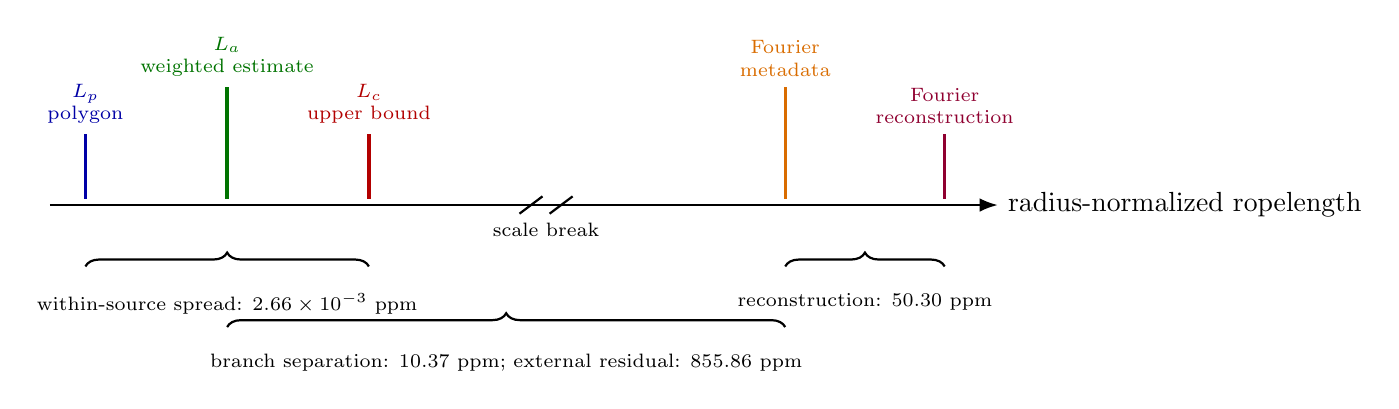
\begin{tikzpicture}[x=2.25cm,y=1cm,>=Latex]
  \draw[thick,->] (0,0)--(5.35,0) node[right] {radius-normalized ropelength};
  \draw[thick] (2.65,-0.11)--(2.78,0.11);
  \draw[thick] (2.82,-0.11)--(2.95,0.11);
  \node[font=\scriptsize,below=3pt] at (2.80,0) {scale break};

  \draw[very thick,blue!65!black] (0.20,0.08)--(0.20,0.90)
    node[above,align=center,font=\scriptsize] {$L_p$\\polygon};
  \draw[very thick,green!45!black] (1.00,0.08)--(1.00,1.50)
    node[above,align=center,font=\scriptsize] {$L_a$\\weighted estimate};
  \draw[very thick,red!70!black] (1.80,0.08)--(1.80,0.90)
    node[above,align=center,font=\scriptsize] {$L_c$\\upper bound};
  \draw[very thick,orange!85!black] (4.15,0.08)--(4.15,1.50)
    node[above,align=center,font=\scriptsize] {Fourier\\metadata};
  \draw[very thick,purple!75!black] (5.05,0.08)--(5.05,0.90)
    node[above,align=center,font=\scriptsize] {Fourier\\reconstruction};

  \draw[decorate,decoration={brace,amplitude=5pt},thick]
    (0.20,-0.78)--(1.80,-0.78)
    node[midway,below=6pt,align=center,font=\scriptsize]
    {within-source spread: $2.66\times10^{-3}$ ppm};
  \draw[decorate,decoration={brace,amplitude=5pt},thick]
    (4.15,-0.78)--(5.05,-0.78)
    node[midway,below=6pt,align=center,font=\scriptsize]
    {reconstruction: $50.30$ ppm};
  \draw[decorate,decoration={brace,amplitude=5pt},thick]
    (1.00,-1.55)--(4.15,-1.55)
    node[midway,below=6pt,align=center,font=\scriptsize]
    {branch separation: $10.37$ ppm; external residual: $855.86$ ppm};
\end{tikzpicture}%
}
\caption{Provenance hierarchy for the high-resolution and Fourier branches.  The horizontal scale is deliberately broken between the high-resolution cluster and the Fourier points.  The weighted value $L_a$ is an estimate, whereas $L_c$ is the reported inscribed-curve upper bound.  The reconstruction point is obtained by re-deriving the centerline length from the stored Fourier coefficients; its separation from the metadata value is roughly five times the metadata--high-resolution branch separation, and still more than an order of magnitude below the external residual.}
\label{fig:provenance-v020}
\end{figure}


Using $L_a/2=16.3714672385$ as the high-resolution diameter-normalized estimate, the unnormalized candidate convention gives
\begin{equation}
  \frac{8\pi}{3}\frac{L_a}{2}=137.1532832132.
\end{equation}
The Fourier metadata branch gives $137.1547054038$, and the Fourier reconstruction branch gives $137.1616038$.  Relative to the external comparison value $137.035999177$, the excesses are $855.86$ ppm, $866.24$ ppm, and $916.58$ ppm, respectively.  The high-resolution--Fourier metadata branch separation is $10.37$ ppm, approximately $82.5$ times smaller than the high-resolution external residual; the metadata--reconstruction separation is $50.30$ ppm, approximately $17$ times smaller.  Geometry provenance matters more than the metadata comparison alone suggests, but even the largest known branch spread is more than an order of magnitude too small to explain the residual.

\begin{table}[t]
\caption{Epistemic status of the high-resolution trefoil length quantities and the Fourier metadata branch.}
\label{tab:provenance-v020}
\begin{ruledtabular}
\scriptsize
\begin{tabular}{@{}lccc@{}}
Quantity & Radius-normalized value & Status & Role\\
\hline
$L_p$ & 32.742934460(1) & polygonal & provenance\\
$L_c$ & 32.742934547(1) & upper bound & conservative\\
$L_a$ & 32.742934477(1) & weighted estimate & central estimate\\
Fourier record & 32.743274000 & rounded metadata & separate branch\\
Fourier reconstruction & 32.744920861 & re-derived from S1 coefficients & diagnostic only\\
\end{tabular}
\end{ruledtabular}
\end{table}

\section{Naturalness and framing-sensitivity diagnostics}
\label{sec:naturalness}

Naturalness is basis dependent, but it is still informative after the operator normalization has been declared.  Suppose, only for diagnosis, that a residual $\Delta=-0.117284$ were assigned entirely to $c_\kappa\calI_{\kappa^2}$.  The required coefficient is shown in \cref{tab:naturalness-curvature}.

\begin{table}[t]
\caption{Coefficient required to close the high-resolution residual using only $c_\kappa\calI_{\kappa^2}$ in the declared normalization.  The middle row is the value returned by the reconstruction diagnostic of Supplementary Code S1; the outer rows bracket it.  The last column shows the shift produced by $c_\kappa=1$.}
\label{tab:naturalness-curvature}
\begin{ruledtabular}
\begin{tabular}{ccc}
$\calI_{\kappa^2}$ & required $c_\kappa$ & shift for $c_\kappa=1$\\
\hline
5     & $-2.35\times10^{-2}$ & 5\\
19.32 & $-6.07\times10^{-3}$ & 19.32\\
33    & $-3.55\times10^{-3}$ & 33\\
\end{tabular}
\end{ruledtabular}
\end{table}

A direct reconstruction of the rounded Fourier record gives $\calI_{\kappa^2}=19.32$, but its high Fourier modes also generate curvature overshoot and it should not be treated as a certified ideal-knot value.  Quantitatively, the reconstruction attains $\hat\kappa_{\max}=2.1668$ against the thickness bound $\hat\kappa\le2$, an excess of $8.3\%$; the reconstructed curve therefore violates the very constraint that defines the tight configuration.  Because $|c_\kappa|=|\Delta|/\calI_{\kappa^2}$, the tabulated value $6\times10^{-3}$ should be regarded as an \emph{optimistic lower estimate} for $|c_\kappa|$, conditional on correcting the curvature overshoot not increasing $\calI_{\kappa^2}$.  The robust statement is the order of magnitude: in this basis a curvature coefficient that closes the residual is around $6\times10^{-3}$.  Without a symmetry or matching mechanism, that is a suppression of roughly two orders relative to unity.  This is not a basis-independent proof of fine tuning, but it weakens the claim that a generic finite-core correction naturally closes a sub-per-mille gap.

Framing introduces an independent sensitivity.  The supplementary reconstruction of the stored Fourier orientation gives $Wr\approx-3.41835$.  Using the Fourier length in the lower bound~\eqref{eq:twist-bound-v020} yields the illustrative values in \cref{tab:framing-sensitivity}.  These are not predictions because no physical self-linking sector has been selected.

\begin{table}[t]
\caption{Illustrative framing sensitivity for the stored Fourier orientation, $Wr\approx-3.41835$ and $\calL_D=16.371637$.  The required coefficient assumes that the entire Fourier-branch residual $-0.118706$ is assigned to the minimum quadratic twist term.}
\label{tab:framing-sensitivity}
\begin{ruledtabular}
\begin{tabular}{ccc}
$SL$ & lower bound on $\calI_{\Omega^2}$ & required $c_\Omega$\\
\hline
$-3$ & 0.422 & $-0.281$\\
$0$  & 28.18 & $-4.21\times10^{-3}$\\
$+3$ & 99.34 & $-1.20\times10^{-3}$\\
\end{tabular}
\end{ruledtabular}
\end{table}

Across the three sectors the inferred coefficient spans a factor of roughly $235$, and the lower bound on $\calI_{\Omega^2}$ spans the same factor.  The mirror sector $SL=+3$ is included because it is the natural companion of $SL=-3$ for the stored orientation and is not excluded by any statement made here.  A centerline alone therefore cannot define a twist correction; the physical framing sector must be fixed before comparison.

\section{Open gauge-stiffness matching and Lorentz universality}
\label{sec:gauge}

Let $a_\mu$ be a dimensionless candidate field with $f_{\mu\nu}=\partial_\mu a_\nu-\partial_\nu a_\mu$.  In a convention where the source term is $\int j^\mu a_\mu$, write
\begin{equation}
  \frac{S_{\rm IR}^{(2)}}{\hbar}
  =-\frac{\Reff}{16\pi}\int f_{\mu\nu}f^{\mu\nu}\,\dd^4\xi
   +\int j^\mu a_\mu\,\dd^4\xi+\cdots.
\end{equation}
Comparison with $-(4g^2)^{-1}\int f^2$ would give $\Reff=4\pi/g^2$.  If $g^2=4\pi\alpha$ in the same charge convention, then $\Reff=\alpha^{-1}$.  Every equality in this chain depends on the normalization of both field and source.

\begin{hypothesis}[Gauge-stiffness matching]
A vortex-tube response can be identified with an inverse electromagnetic coupling only if one microscopic model independently establishes
\begin{enumerate}[label=(\alph*)]
  \item a protected $U(1)$ redundancy or equivalent first-class constraint;
  \item exactly two gapless physical transverse modes and no physical longitudinal mode;
  \item a conserved current with fixed unit-charge normalization;
  \item the same coupling in static and radiative sectors;
  \item positive energy and stable propagation;
  \item an isotropic infrared dispersion $\omega^2=c_{\rm eff}^2k^2+O(k^4)$ for both polarizations;
  \item one Lorentz-invariant infrared causal cone shared by the gauge modes and the matter probes used to define the coupling;
  \item no use of the target coupling or equivalent target-dependent calibration in determining the response.
\end{enumerate}
\end{hypothesis}

An incompressible medium has a preferred microscopic frame.  Effective Lorentzian metrics and relativistic-looking propagation can emerge in analogue systems, but preferred-frame corrections, dispersion, and multiple effective cones are separate obstructions \cite{BarceloLiberatiVisser2026}.  Consequently, two transverse modes and a Maxwell-shaped quadratic term are not sufficient.

\subsection{Field-rescaling obstruction}

Under $a_\mu\mapsto\lambda a_\mu$ and $j^\mu\mapsto j^\mu/\lambda$, the source term is unchanged while the coefficient assigned to $f^2$ changes.  The kinetic coefficient is therefore not an observable coupling until the current normalization is fixed independently.

\section{Independent calibration and falsification protocol}
\label{sec:calibration}

The leading normalization must be calibrated or derived independently before the finite-core residual is defined.  For calibration configuration $n$, write
\begin{equation}
  y_n:=\Rmicro[\gamma_n,f_n,\Omega_{3,n}]
      -\ZL(\mu)\calL_{D,n}
      -\Rnl[\gamma_n,f_n;\mu].
  \label{eq:calibration-v020}
\end{equation}
Only after the logarithmic/nonlocal part has been frozen may a local regression be attempted:
\begin{equation}
  y_n=\sum_aA_{na}c_a+\varepsilon_n.
\end{equation}
A phenomenological comparison using $\ZL=8\pi/3$ is permissible only when labeled as a preregistered convention rather than a derived coefficient.

The calibration set should include circular rings over several $R/D$, straight periodically twisted tubes, antiparallel finite-core pairs at several separations, and mixed geometries held out from fitting.  Since the tight trefoil is outside a controlled slender-curvature regime, the full regularized functional should be evaluated whenever possible rather than inferred from three local features.


\begin{figure}[t]
\centering
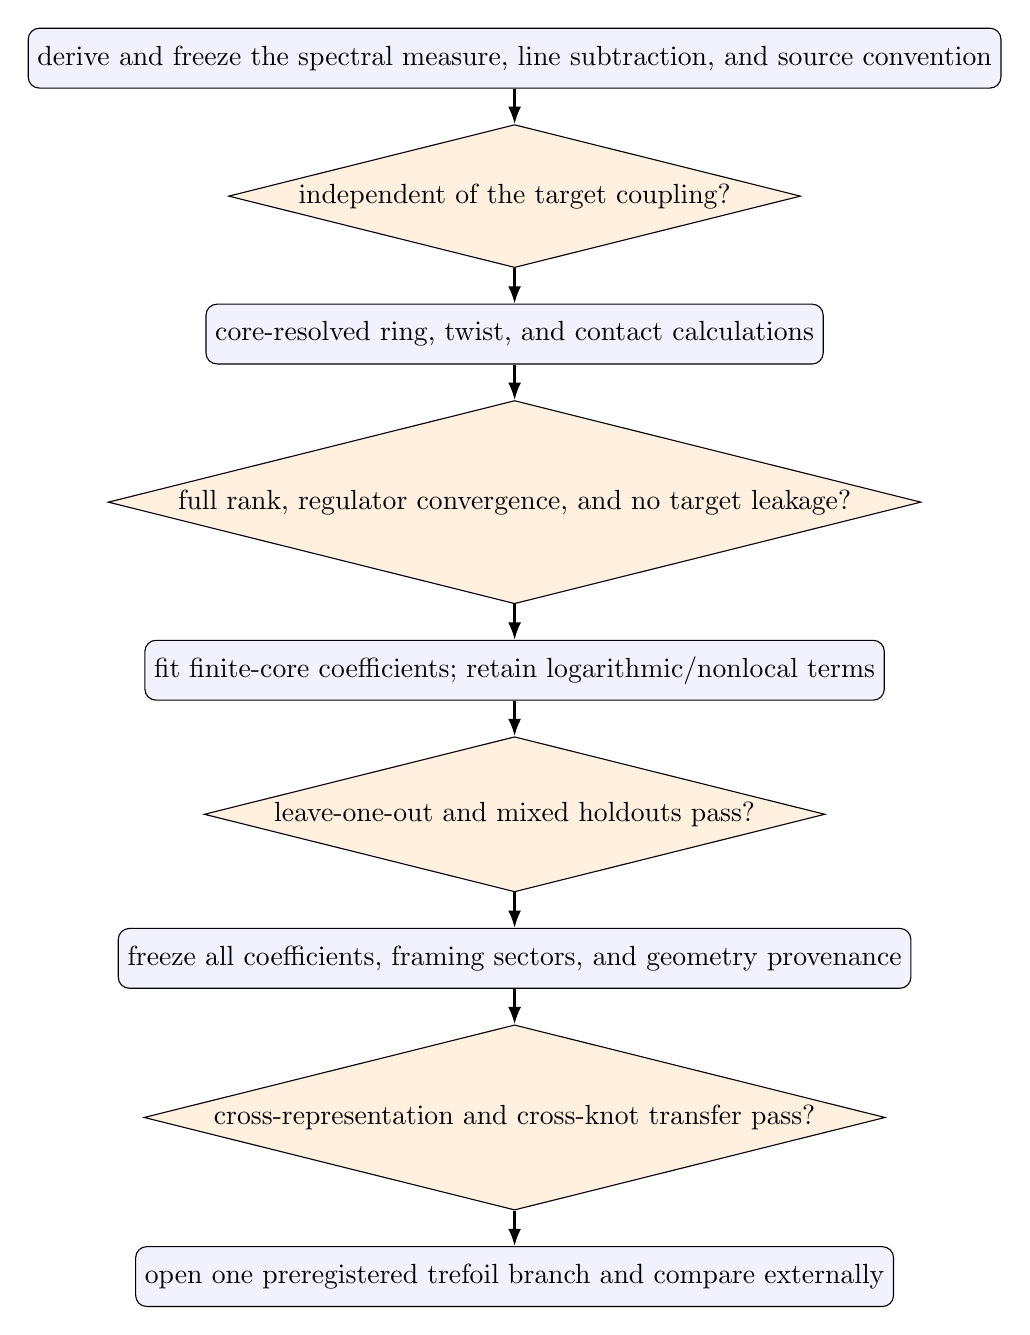
\begin{tikzpicture}[
  node distance=4.5mm,
  stagebox/.style={draw,rounded corners,minimum width=7.4cm,minimum height=0.76cm,align=center,fill=blue!5},
  gate/.style={draw,diamond,aspect=4,align=center,fill=orange!12,inner sep=1.5pt},
  arr/.style={-{Latex[length=2.2mm]},thick}
]
  \node[stagebox] (z) {derive and freeze the spectral measure, line subtraction, and source convention};
  \node[gate,below=of z] (gz) {independent of the target coupling?};
  \node[stagebox,below=of gz] (a) {core-resolved ring, twist, and contact calculations};
  \node[gate,below=of a] (g0) {full rank, regulator convergence, and no target leakage?};
  \node[stagebox,below=of g0] (b) {fit finite-core coefficients; retain logarithmic/nonlocal terms};
  \node[gate,below=of b] (g1) {leave-one-out and mixed holdouts pass?};
  \node[stagebox,below=of g1] (c) {freeze all coefficients, framing sectors, and geometry provenance};
  \node[gate,below=of c] (g2) {cross-representation and cross-knot transfer pass?};
  \node[stagebox,below=of g2] (d) {open one preregistered trefoil branch and compare externally};
  \draw[arr] (z)--(gz); \draw[arr] (gz)--(a); \draw[arr] (a)--(g0);
  \draw[arr] (g0)--(b); \draw[arr] (b)--(g1); \draw[arr] (g1)--(c);
  \draw[arr] (c)--(g2); \draw[arr] (g2)--(d);
\end{tikzpicture}
\caption{Revised calibration and falsification sequence.  The normalization of the leading length term is itself part of the independent matching problem; it is not supplied by the angular identity.}
\label{fig:calibration-v020}
\end{figure}


The external coupling, elementary charge, final target residual, and any parameter already calibrated through that coupling are forbidden calibration inputs.  At minimum the programme requires target exclusion, full-rank identifiability, resolution and regulator convergence, leave-one-out success, mixed holdouts, cross-representation transfer, cross-knot transfer, frozen framing sectors, and one preregistered final comparison.

\section{Discussion}
\label{sec:discussion}

The exact part of the argument is narrower than the original formulation.  Spatial isotropy fixes the mean transverse fraction $2/3$.  The number $8\pi/3$ is the same identity integrated with the unnormalized area measure on the unit sphere.  A physical response coefficient requires the full measure and normalization of the underlying modes.  The angular identity alone does not provide them.

The tube-volume calculation supplies a useful local no-go result, but its prefactor does not independently derive the same coefficient.  Finite-core energetics begins with the singular Biot--Savart functional and introduces a logarithmic self-energy, profile-dependent constants, long-range induction, and contact.  The tight trefoil is not in the small-$D\kappa$ regime, so a low-order local operator series has no automatic hierarchy.

The naturalness table makes the numerical issue explicit.  In the declared curvature basis, generic coefficients of order unity would produce corrections much larger than the observed sub-per-mille residual.  Matching the residual requires suppressed coefficients or cancellations.  Such suppression may be physically real, but it must be derived; it cannot be inferred from numerical proximity.

Helicity remains valuable because it constrains the exchange between writhe and material twist.  However, the self-linking sector is additional physical data.  The same centerline can support very different minimum quadratic twist energies in different framings.

Finally, an electromagnetic interpretation is a much stronger statement than transversality.  It requires gauge redundancy, current normalization, static--radiative equality, and emergent Lorentz universality.  Until those conditions and the full finite-core response are derived together, the trefoil comparison is best understood as a normalization-dependent geometric coincidence that motivates a falsification programme.

\section{Conclusions}

The revision supports the following conclusions:
\begin{enumerate}[leftmargin=*]
  \item The exact invariant statement is the normalized isotropic mean
  \[
    \langle t_iP_{ij}t_j\rangle_{S^2}=2/3.
  \]
  The value $8\pi/3$ is the corresponding unnormalized angular integral.
  \item The coefficient of a physical length operator is an open matching parameter $\ZL(\mu)$; choosing $8\pi/3$ is a convention until the complete spectral measure is derived.
  \item The bare local projector and constant circular tube volume generate no curvature correction.
  \item Finite-core vortex energy contains logarithmic and nonlocal contributions.  A polynomial three-operator expansion is not controlled on curvature-limited portions of the tight trefoil.
  \item The rule $c_L=0$ is a preregistered subtraction convention, not a derivation of the line coefficient.
  \item Helicity constrains a parity-even quadratic twist energy, but the result depends strongly on the chosen self-linking sector.
  \item The high-resolution quantities $L_p$, $L_c$, and $L_a$ have different epistemic status.  The known geometry-branch spread is much smaller than the external residual.
  \item In the declared operator normalization, closing the residual requires suppressed coefficients unless a specific cancellation or symmetry is derived.
  \item Identifying the response with an inverse electromagnetic coupling remains open and additionally requires Lorentz universality of the infrared gauge and matter sectors.
\end{enumerate}

The scientifically decisive next step is a core-resolved calculation that derives the spectral measure, line subtraction, logarithmic self-energy, framing sector, and source normalization without consulting the external coupling.  Until then, the numerical proximity should not be presented as a prediction.

\begin{acknowledgments}
The author thanks the developers of the mathematical and numerical ropelength literature for making high-resolution knot geometries and contact diagnostics available.  The present version is self-contained and relies only on the literature and supplementary data explicitly cited here.
\end{acknowledgments}

\appendix

\section{Supplementary Fourier reconstruction checks}
\label{app:fourier-reconstruction}

Supplementary Code S1 reconstructs the trefoil record
\begin{equation}
  \bm X(t)=\sum_n\left[\bm A_n\cos(nt)+\bm B_n\sin(nt)\right]
\end{equation}
from Supplementary Data S1.  The rounded coefficients reproduce a length
\begin{equation}
  \calL_D^{\rm rec}=16.3724604307,
\end{equation}
i.e.\ $50.30$ ppm above the metadata value $16.371637$ and $60.67$ ppm above the high-resolution estimate $L_a/2=16.3714672385$, and they generate local curvature overshoot, $\hat\kappa_{\max}=2.1668$ against the thickness bound $\hat\kappa\le2$.  The metadata length is therefore retained for the scalar branch while reconstructed geometry is used only for diagnostics.  Both numbers are reported so that the reconstruction can be checked independently and so that the provenance hierarchy of \cref{fig:provenance-v020} is complete rather than restricted to the two branches that happen to agree most closely.

A midpoint discretization of the Gauss writhe integral converges for the stored orientation toward
\begin{equation}
  Wr\approx-3.41835.
\end{equation}
The sign changes under reversal or mirroring.  The quoted value is an orientation-specific diagnostic of the rounded Fourier record, not a universal writhe assigned to every ideal-trefoil representation.

\section{Schematic contact functional}

A numerical contact diagnostic may be defined using a nonnegative shell kernel $K_\sigma(R)$ concentrated near normalized separation $R=1$ and an orthogonality weight $Q_\eta$:
\begin{align}
  \calC_{\rm contact}[\gamma]
  =\frac12\int\!\dd\sigma\int\!\dd\sigma'\,
  &K_\sigma(|\bm X(\sigma)-\bm X(\sigma')|)\\
  &\times Q_\eta(\unitvec{R}\cdot\bm t(\sigma),
                  \unitvec{R}\cdot\bm t(\sigma')).
\end{align}
This is a regulator-dependent diagnostic, not a topological invariant.  Its widths, exclusions, and core profile must be frozen before calibration.

\section{Gauge-field rescaling}

Starting from
\begin{equation}
  S[a,j]=-\frac{1}{4g^2}\int f^2+\int j\cdot a,
\end{equation}
set $a'=\lambda a$ and $j'=j/\lambda$.  Then
\begin{equation}
  S[a',j']=-\frac{1}{4(\lambda g)^2}\int f'^2+\int j'\cdot a'.
\end{equation}
The numerical coupling changes unless the source normalization is independently fixed.

\begin{thebibliography}{99}

\bibitem{CantarellaKusnerSullivan2002}
J.~Cantarella, R.~B.~Kusner, and J.~M.~Sullivan,
``On the minimum ropelength of knots and links,''
\emph{Invent. Math.} \textbf{150}, 257--286 (2002),
\href{https://doi.org/10.1007/s00222-002-0234-y}{doi:10.1007/s00222-002-0234-y}.

\bibitem{AshtonCantarellaPiatekRawdon2011}
T.~Ashton, J.~Cantarella, M.~Piatek, and E.~J.~Rawdon,
``Knot tightening by constrained gradient descent,''
\emph{Exp. Math.} \textbf{20}, 57--90 (2011),
\href{https://doi.org/10.1080/10586458.2011.544581}{doi:10.1080/10586458.2011.544581}.

\bibitem{PrzybylPieranski2014}
S.~Przybyl and P.~Pieranski,
``High resolution portrait of the ideal trefoil knot,''
\emph{J. Phys. A: Math. Theor.} \textbf{47}, 285201 (2014),
\href{https://doi.org/10.1088/1751-8113/47/28/285201}{doi:10.1088/1751-8113/47/28/285201}.

\bibitem{Saffman1992}
P.~G.~Saffman,
\emph{Vortex Dynamics}
(Cambridge University Press, Cambridge, 1992),
\href{https://doi.org/10.1017/CBO9780511624063}{doi:10.1017/CBO9780511624063}.

\bibitem{HornNicolisPenco2015}
B.~Horn, A.~Nicolis, and R.~Penco,
``Effective string theory for vortex lines in fluids and superfluids,''
\emph{J. High Energy Phys.} \textbf{2015}, 153 (2015),
doi:\href{https://doi.org/10.1007/JHEP10(2015)153}{10.1007/JHEP10(2015)153}.

\bibitem{Moffatt1969}
H.~K.~Moffatt,
``The degree of knottedness of tangled vortex lines,''
\emph{J. Fluid Mech.} \textbf{35}, 117--129 (1969),
\href{https://doi.org/10.1017/S0022112069000991}{doi:10.1017/S0022112069000991}.

\bibitem{MoffattRicca1992}
H.~K.~Moffatt and R.~L.~Ricca,
``Helicity and the C\u{a}lug\u{a}reanu invariant,''
\emph{Proc. R. Soc. Lond. A} \textbf{439}, 411--429 (1992),
\href{https://doi.org/10.1098/rspa.1992.0159}{doi:10.1098/rspa.1992.0159}.

\bibitem{ChuiMoffatt1995}
A.~Y.~K.~Chui and H.~K.~Moffatt,
``The energy and helicity of knotted magnetic flux tubes,''
\emph{Proc. R. Soc. Lond. A} \textbf{451}, 609--629 (1995),
\href{https://doi.org/10.1098/rspa.1995.0146}{doi:10.1098/rspa.1995.0146}.

\bibitem{MaggioniRicca2009}
F.~Maggioni and R.~L.~Ricca,
``On the groundstate energy of tight knots,''
\emph{Proc. R. Soc. A} \textbf{465}, 2761--2783 (2009),
\href{https://doi.org/10.1098/rspa.2008.0536}{doi:10.1098/rspa.2008.0536}.

\bibitem{MaggioniEtAl2009}
F.~Maggioni, S.~Z.~Alamri, C.~F.~Barenghi, and R.~L.~Ricca,
``Kinetic energy of vortex knots and unknots,''
\emph{Nuovo Cimento C} \textbf{32}, 133--142 (2009),
\href{https://doi.org/10.1393/ncc/i2009-10351-6}{doi:10.1393/ncc/i2009-10351-6}.

\bibitem{MaggioniEtAl2010}
F.~Maggioni, S.~Alamri, C.~F.~Barenghi, and R.~L.~Ricca,
``Velocity, energy, and helicity of vortex knots and unknots,''
\emph{Phys. Rev. E} \textbf{82}, 026309 (2010),
\href{https://doi.org/10.1103/PhysRevE.82.026309}{doi:10.1103/PhysRevE.82.026309}.

\bibitem{BuniyKephart2005}
R.~V.~Buniy and T.~W.~Kephart,
``Glueballs and the universal energy spectrum of tight knots and links,''
\emph{Int. J. Mod. Phys. A} \textbf{20}, 1252--1259 (2005),
\href{https://doi.org/10.1142/S0217751X05024146}{doi:10.1142/S0217751X05024146}.

\bibitem{BuniyEtAl2014}
R.~V.~Buniy, J.~Cantarella, T.~W.~Kephart, and E.~J.~Rawdon,
``Tight knot spectrum in QCD,''
\emph{Phys. Rev. D} \textbf{89}, 054513 (2014),
\href{https://doi.org/10.1103/PhysRevD.89.054513}{doi:10.1103/PhysRevD.89.054513}.

\bibitem{Calugareanu1961}
G.~C\u{a}lug\u{a}reanu,
``Sur les classes d'isotopie des noeuds tridimensionnels et leurs invariants,''
\emph{Czech. Math. J.} \textbf{11}, 588--625 (1961).

\bibitem{White1969}
J.~H.~White,
``Self-linking and the Gauss integral in higher dimensions,''
\emph{Am. J. Math.} \textbf{91}, 693--728 (1969),
\href{https://doi.org/10.2307/2373348}{doi:10.2307/2373348}.

\bibitem{Antman2005}
S.~S.~Antman,
\emph{Nonlinear Problems of Elasticity}, 2nd ed.
(Springer, New York, 2005),
\href{https://doi.org/10.1007/0-387-27649-1}{doi:10.1007/0-387-27649-1}.

\bibitem{BarceloLiberatiVisser2026}
C.~Barcel\'o, S.~Liberati, and M.~Visser,
``Analogue gravity,''
\emph{Living Rev. Relativ.} \textbf{29}, 2 (2026),
\href{https://doi.org/10.1007/s41114-026-00064-9}{doi:10.1007/s41114-026-00064-9}.

\bibitem{TiesingaEtAl2024}
E.~Tiesinga, P.~J.~Mohr, D.~B.~Newell, and B.~N.~Taylor,
``The 2022 CODATA recommended values of the fundamental physical constants,''
NIST Standard Reference Database 121, Web Version 9.0 (2024),
\url{https://physics.nist.gov/constants}.

\end{thebibliography}

\end{document}